% !TeX spellcheck = de_DE

\subsection{Trainingsumgebung}
Im Folgenden soll der Aufbau der Trainingsumgebung beschrieben werden, welche es erlaubt verschiedenste Kreaturen ohne große Anpassungen zu trainieren. Im Laufe der Projektgruppe wurden drei unterschiedliche Versionen der Trainingsumgebung genutzt. 

\subsubsection{Vorherige Versionen}
Die erste Version ist eine leicht abgeänderte Form der ML-Agents-Beispielumgebung für den Walker. Dabei handelt es sich um eine Unity-Szene mit einer fest vorgebenden Anzahl an Arenen und Kreaturen, welche trainiert werden können.

Da sich hier schnell Limitationen in Bezug auf die Anpassbarkeit herausstellten wurde die Umgebung geändert, so dass die Anzahl der Arenen dynamisch generiert werden und Kreaturen als Prefab und per Seed über den \texttt{CreatureGenerator} platziert werden können. 

Die  \texttt{DynamicEnviormentGenerator}-Umgebung ist dabei aus den folgenden Klassen aufgebaut:

\begin{itemize}
	\item \texttt{DynamicEnviormentGenerator}
	\begin{itemize}
		\item \texttt{TerrainGenerator} %Todo change when replaced by package
		\item Verschiedenen Konfigurationsdateien
		\item \texttt{DebugScript}
	\end{itemize}
	\item großteils alle modifizierten ML-Agents Skripten
\end{itemize} 

Da die Umgebung weiterhin als zusätzliche Szene in dem Projekt existiert\footnote{Es sei dabei angemerkt, dass die Szene nicht aktiv getestet wird und deswegen nicht garantiert werden kann, dass mit weiteren Änderungen die Funktionalität bestehen bleibt.} und die aktuelle Version der Trainingsumgebung auf dem \texttt{DynamicEnviormentGenerator} aufbaut, wird im Folgenden auf den Aufbaue des \texttt{DynamicEnviormentGenerator} sowie dessen Hilfsklassen eingegangen. Die Hilfsklassen sind der \texttt{TerrainGenerator}, \texttt{GenericConfig} und dessen Implementierungen sowie das \texttt{DebugScript}. Erstere ist verantwortlich für die Generierung des Terrains, die Config-Dateien laden dynamisch die Einstellungen aus einer Datei und das letzte Skript beinhaltet hilfreiche Debug-Einstellungen. Die grundsätzliche Idee der Trainingsumgebung stammt von dem ML-Agents-Walker. Da an diesem keine Versuche mit Unterschiedlichen Umgebungen und Kreaturen durchgeführt wurden, ist der Aufbau des Projekts nicht dynamisch genug. 

\paragraph{Dynamic Enviorment Generator}
\begin{figure}
	\centering
	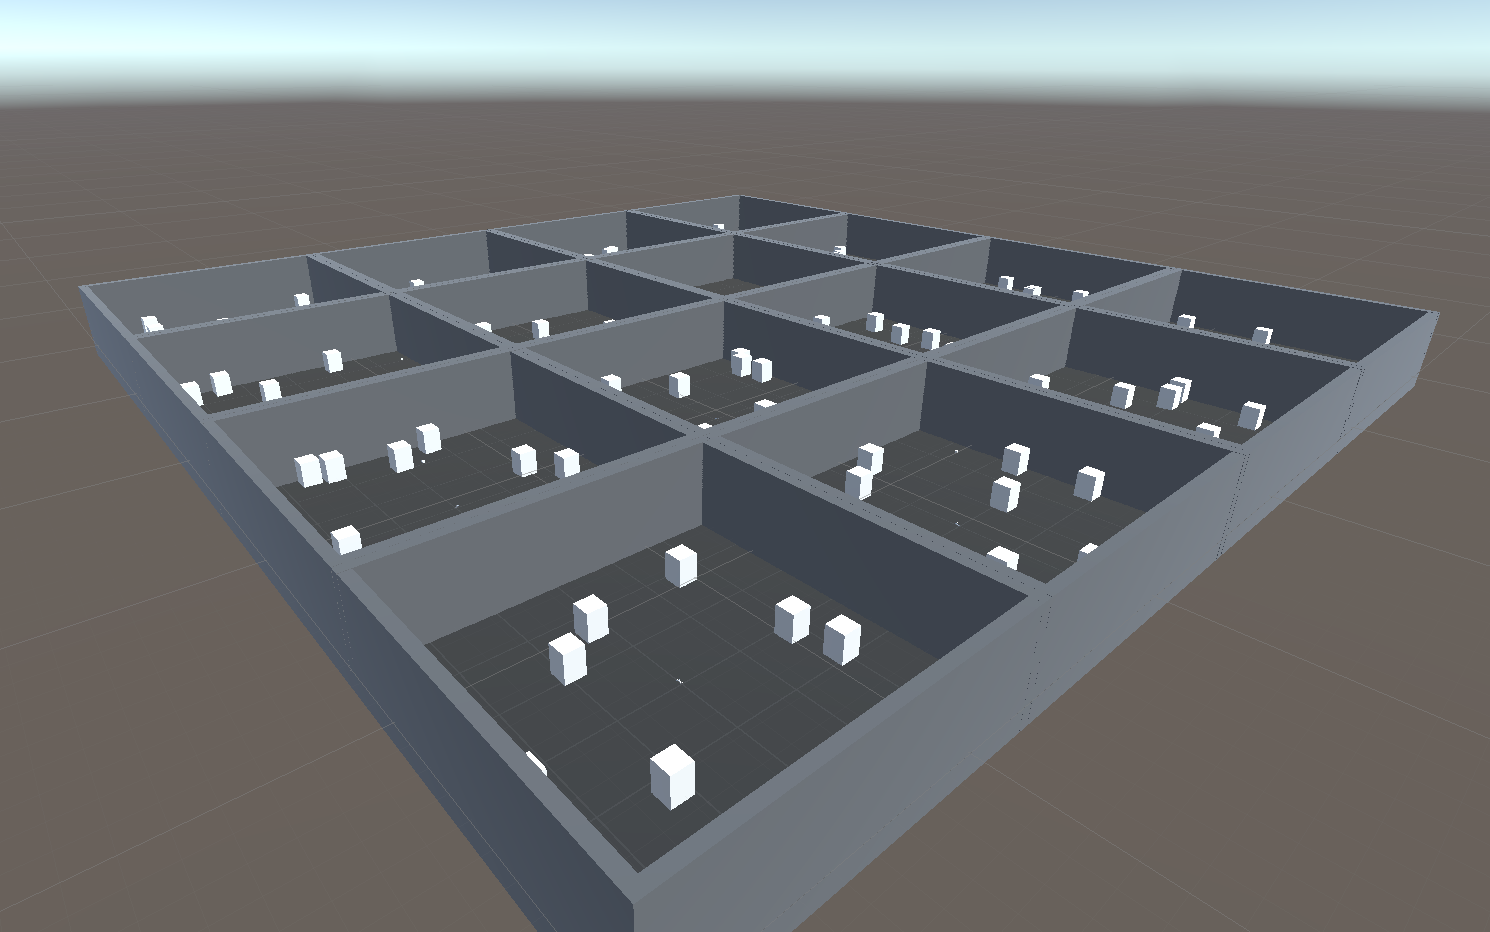
\includegraphics[width=0.7\linewidth]{resources/img/DEGArenen}
	\caption[Beispiel der generierten Trainingsumgebung]{Ein Beispiel der generierten Trainingsumgebung mit mehreren Arenen.}
	\label{bspArena}
\end{figure}
Zur dynamischen Umsetzung der Trainingsarena werden alle Objekte zur Laufzeit erstellt. Die Generierung der Arena läuft dann wie folgt ab:
\begin{enumerate}
	\item Erstellen von $n$ Arenen, wobei $n$ eine zu setzende Variable ist. 
	\item Füge ein Ziel für die Kreatur in die Arena ein
	\item Generiere die Kreatur
\end{enumerate} 
Die einzelnen (Teil)-Arenen, abgebildet in der Grafik \ref{bspArena}, bestehen aus einem Container-Objekt unter dem ein Terrain und vier Wall-Prefabs angeordnet sind. Diese Prefabs und weitere Elemente wie Texturen werden dynamisch aus einem Ressourcen-Ordner geladen, damit möglichst wenige zusätzliche Konfigurationen den Editor verkomplizieren. Das Terrain wird mit leeren Terraindaten vorinitialisiert und später befüllt. Hierbei kann die Position des Container-Objects in der Szenen wie folgt berechnet werden:
\begin{align}
	\begin{pmatrix}
	\lceil \frac{\text{Anzahl der Arenen}}{\sqrt{\text{Anzahl der Arenen}}} \rceil \\
	0 \\
	\text{Anzahl der Arenen} \mod \sqrt{\text{Anzahl der Arenen}} \\
	\end{pmatrix}
	 = 	\begin{pmatrix}
	 x  \\
	 y \\
	 z  \\
	 \end{pmatrix}
\end{align}
Alle anderen Objektpositionen müssen danach neu im lokalen Koordinatensystem gesetzt werden. Da die Unity-Standard-Texturen sehr hell sind sind, werden die Texturen bei der Initialisierung mit ML-Agents-Texturen, welche dunkler sind, getauscht. An das Terrain werden zuletzt Collider und ein \texttt{TerrainGenerator}-Skript angefügt. 

In Schritt 2. der Arenagenerierung muss beachtet werden, dass nach dem Erstellen des Zielobjekts das \texttt{WalkTargetScript} hinzugefügt wird. Am Ende des Erstellungsprozesses wird der Walker erstellt. Hierzu wird ein von den Creature-Generator-Team bereitgestelltes Paket\footnote{https://github.com/PG649-3D-RPG/Creature-Generation} benutzt. Das Paket stellt ein Klasse bereit, welche mit zwei Skript-Objekte konfiguriert wird. Zusätzlich wird ein seed übergeben, welcher reproduzierbare Kreaturen erlaubt. Die erstelle Kreatur muss danach mit den entsprechenden ML-Agent-Skripten versehen werden. Hierzu wird ein \texttt{WalkerAgent} Objekt als String übergeben. Dies ermöglicht es, mehrere unterschiedliche Agent-Skripte durch eine Änderung im Editor zu setzen. Somit können Reward-Funktion und Observation für zwei unterschiedliche Trainingsversuche getrennt, in eigenen Dateien, entwickelt werden.

\paragraph{TerrainGenerator}
Da ein typisches Spieleterrain im Gegensatz zum ML-Agents-Walker-Terrain nicht flach ist, wurde ein neues Objekt erstellt, welches sowohl die Generierung von Hindernissen, als auch eines unebenen Bodens erlaubt. Um ein möglichst natürlich erscheinendes Terrain zu erzeugen wird ein Perlin-Noise verwendet. Dieses spiegelt jeweils die Höhe des Terrains an einen spezifischen Punkt wider. Im späteren Projektverlauf wurde dieses Skript durch den Terraingenerator des dazugehörigen Teams ersetzt.

\paragraph{Konfigurationsobjekte}
Da sich die statische Konfiguration des ML-Agents-Walker als problematisch erwies, wurde die Konfiguration über die Laufzeit des Projekts dynamischer gestaltet. Zuerst wurden alle Konfigurationen im \texttt{DynamicEnviormentGenerator} gespeichert. Was unübersichtlich war und zu ständigen neubauen des Projektes führte. Deshalb wurde eine \texttt{GenericConfig} Klasse eingeführt, welche die im Editor eingestellten Optionen für die einzelnen Teilbereiche Terrain, Arena und ML-Agent in Json-Format in den Streaming-Asset-Ordner speichert. Da dieser Ordner beim bauen des Projekts in das fertige Spiel übertragen wird, sind diese Konfigurationen automatisiert dort vorhanden. 

Im Fall, dass das Spiel ohne Editor gestartet wird, was meist beim Training der Fall ist, lädt das generische Objekt aus den Json-Dateien die Einstellungen und ersetzt die Editorkonfiguration damit. Hierdurch ist ein ändern der Konfiguration des Spiels ohne neu-erstellen der Binärdateien ermöglicht. Diese Konfigurationsart fügt Abhängigkeiten zu dem Unity eigenen JsonUtility\footnote{https://docs.unity3d.com/ScriptReference/JsonUtility.html} hinzu. Die Konfigurationsmöglichkeiten sind in der Grafik \ref{bspDEGOptionen} zu sehen.

\begin{figure}
	\centering
	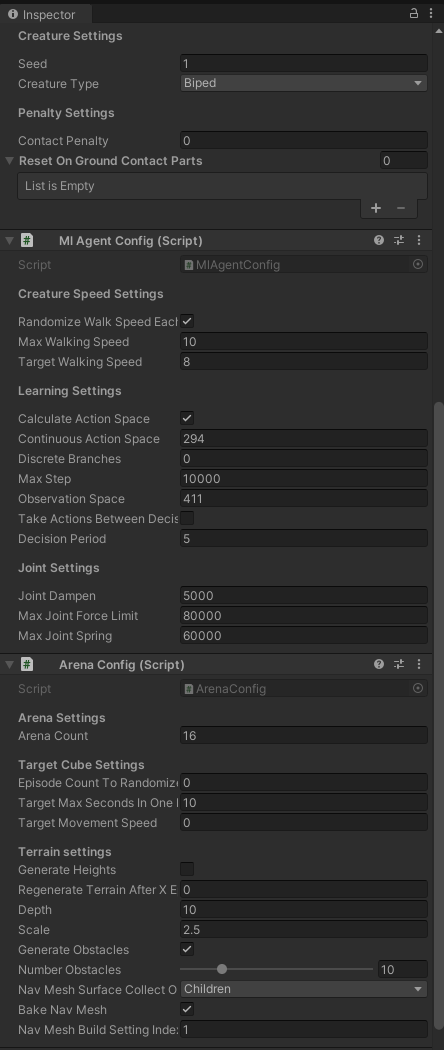
\includegraphics[width=0.4\linewidth]{resources/img/DEGConfig}
	\caption[Konfigurationsmöglichkeiten des \texttt{DynamicEnviormentGenerator}]{Konfigurationsmöglichkeiten des \texttt{DynamicEnviormentGenerator} im Unity-Editor.} 
	\label{bspDEGOptionen}
\end{figure}

\subsubsection{Aktuelle Version -- AdvancedEn}
\begin{figure}
	\centering
	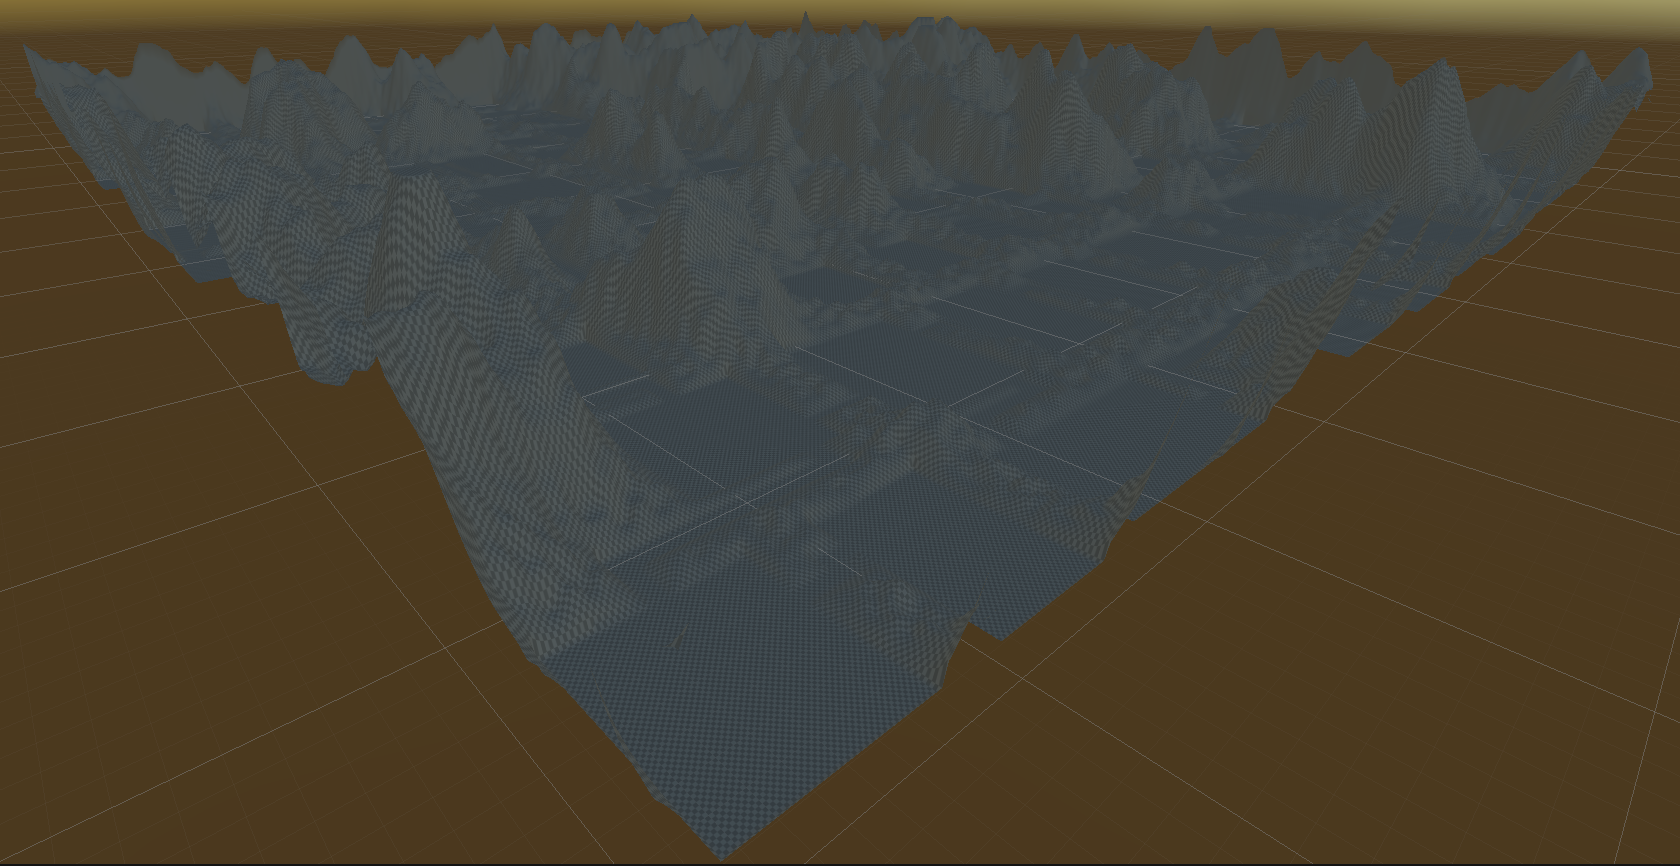
\includegraphics[width=0.7\linewidth]{resources/img/AEGArena.png}
	\caption[Konfigurationsmöglichkeiten des \texttt{AdvancedEnviormentGenerator}]{Ansicht der generierten Arena durch den \texttt{AdvancedEnviormentGenerator}.} 
	\label{bspAEGArena}
\end{figure}

Über den Produktzyklus des \texttt{DynamicEnviormentGenerator} sind insbesondere gegen Ende der Projektgruppe mehre Probleme aufgefallen. Da durch häufige Updates die Codequalität nachlässt und einige zuvor bedachte Optionen durch Zeitmangel nicht mehr relevant waren wurde entschieden, die Umgebung durch eine neue zu ersetzen. Dabei wurde insbesondere auf eine starke nähe zum Spiel geachtet, damit nur wenige Modifikationen für dieses erstellt werden müssen.

Die neue Umgebung wird im folgenden als \texttt{AdvancedEnviormentGenerator} bezeichnet und befindet sich in einer neuen Szene mit den Namen \enquote{AdvancedMovementScene}. Bedingt durch die konzeptionelle Weiterentwicklung der vorherigen Versionen mussten in den restlichen Skripten kaum Anpassungen durchgeführt werden. Eine Hauptänderung ist der geringeren Anzahl an verweisen auf den neuen Generator. Da der \texttt{DynamicEnviormentGenerator} in seinen ersten Versionen eine Art Gottklasse war, verwiesen die meisten andere Skripte darauf. Dies führte schnell zu unübersichtlichen Abhängigkeiten.

Die Generator-Klasse selbst konnte deutlich gekürzt werden, da eine Generierung von Arenen nicht mehr benötigt wird. Zu dem Zeitpunkt der Erstellung existierte bereits der \texttt{TerrainGenerator} für das finale Spiel, welche ab dieser Version für die Trainingsumgebung verwendet wird. Weiterhin ermöglichte dies eine Entfernung von vielen Einstellungen für das Terrain aus dem Generator-Objekt.

In der Abbildung \ref{bspAEGArena} ist das Endergebnis des \texttt{AdvancedEnviormentGenerator} dargestellt. Da es im realen Spiel zu Kollisionen zwischen verschiedenen Kreaturen kommen kann, wurde für die Trainingsumgebung nur eine zusammenhängende Arena verwendet. Insgesamt stimmen die Bedingungen für das Lernen und dem Spiel somit überein, da wie im Spiel kleine Korridore und Arenen mit ggf. mehreren Kreaturen genutzt werden.
\subsection{Erweiterung der Agent-Klasse}
\todo{texttt im Titel?}

\begin{figure}
	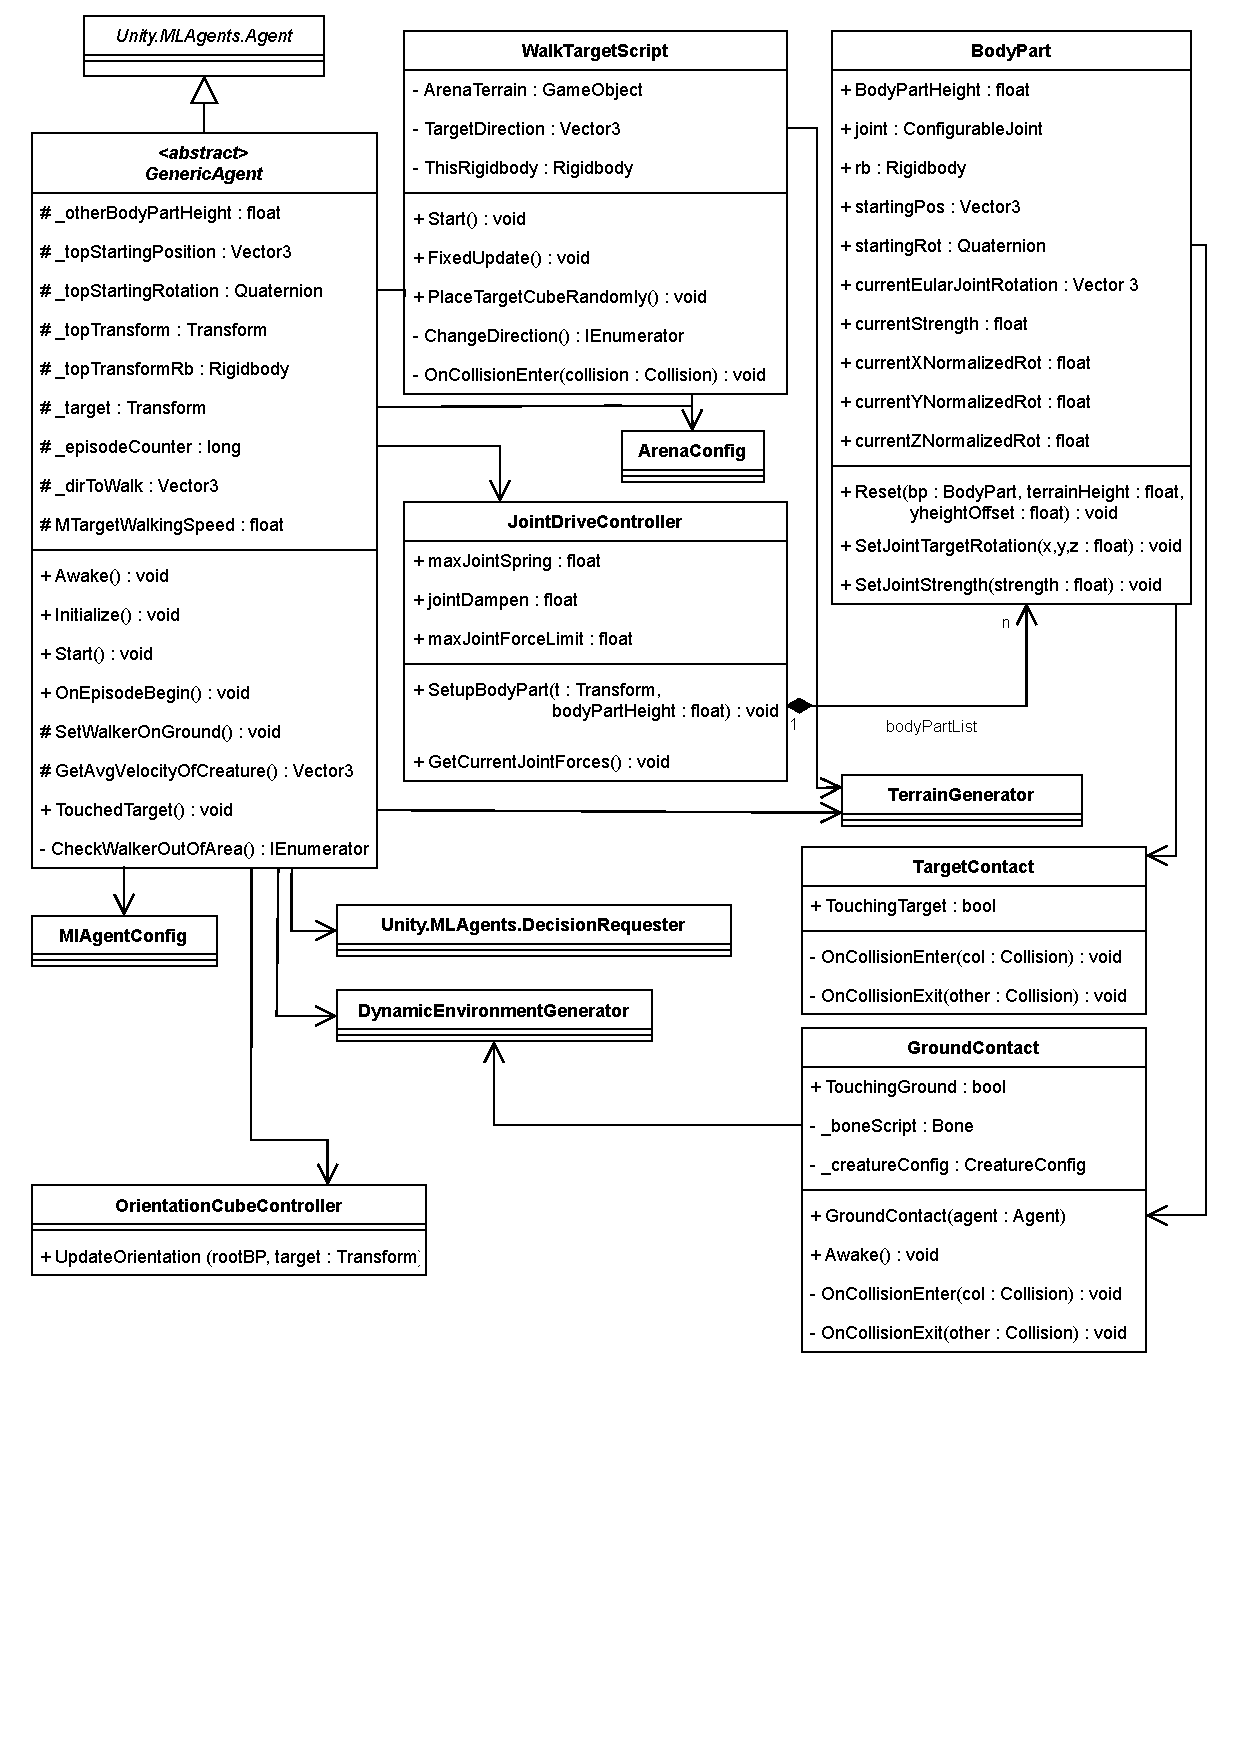
\includegraphics[width=\textwidth, trim={0cm 6.5cm 0cm 0cm}, clip]{resources/img/PG_Agent.drawio.pdf}
	\caption{UML-Diagram der GenericAgent-Klasse und weitere relevante Klassen}
	\label{fig:umlAgent}
\end{figure}

Als eine Erweiterung der \texttt{Agent}-Klasse von ML-Agents stellt die \texttt{GenericAgent}-Klasse das Verbindungsst"uck zwischen dem ML-Framework und der Unity-Engine dar. Im Folgenden wird der Aufbau der Klasse \texttt{GenericAgent} sowie derer Hilfsklassen \texttt{JointDrive\-Controller}, \texttt{BodyPart}, \texttt{OrientationCubeController} und \texttt{WalkTargetScript} erläutert und die Funktionalität dieser Klassen erklärt. Zur Veranschaulichung befindet sich in Abbildung \ref{fig:umlAgent} ein UML-Diagram. Der Aufbau dieser Klassen orientiert sich dabei sehr stark an die Implementierung des ML-Agents Walker.

\subsubsection{GenericAgent}

Die kontrollende Instanz einer konkreten Trainingsumgebung ist die \texttt{GenericAgent}-Klasse. Diese ist dazu in der Lage, mit dem Modell des ML-Frameworks zu interagieren, also sowohl Beobachtungen der Trainingsumgebung weiterzugeben also auch die Ausgaben des Modells anzunehmen (und zu verarbeiten). Außerdem ist die Klasse f"ur die Instandhaltung der Trainingsumgebung verantwortlich, indem sie Events der Umgebung verarbeitet (z.B. das Erreichen des Targets oder das Verlassen des zugänglichen Bereiches) und ggf. spezifizierte Routinen wie das Zur"ucksetzen der Umgebung durf"uhrt.
Schließlich muss die \texttt{GenericAgent}-Klasse noch die Rewards f"ur die Trainingsumgebung verteilen. Zu diesem Zweck ist die Klasse als \textit{abstract} definiert, da diese Rewardfunktionen stark von der Aufgabe des Agents abhängig sind. So benötigt zum Beispiel ein Agent, welcher ein bestimmtest Ziel möglichst schnell erreichen soll eine andere Reward-Funktion als ein Agent, welcher sich möglichst gut vor dem Spieler verstecken soll. Verschiedene Agents können so ohne Redundanz einfach als eine Erweiterung der \texttt{GenericAgent}-Klasse implementiert werden.

\todo{Mehr auf Reward-Funktionen eingehen oder erst bei konkreten Agents?}

\subsubsection{JointDriveController und BodyPart}

Um die Ingame-Repräsentation (also die generierte Creature) des Agents zu kontrollieren, besitzt der \texttt{GenericAgent} einen \texttt{JointDriveController}. Bei der Initialisierung der Trainingsumgebung wrappt der \texttt{JointDriveController} die verschiedenen Unity-Transforms der Creature in Instanzen der Hilfsklasse \texttt{BodyPart}. Die Klasse \texttt{BodyPart} gibt uns leichten Zugang zu häufig benötigten Funktionalitäten, wie zum Beispiel das Zur"ucksetzen oder Steuern des Transform. Auch besitzt ein \texttt{BodyPart} n"utzliche Informationen "uber das jeweilige Transform, welche dem ML-Modell weitergegeben werden können. Nach der Initialisierung stellt der \texttt{JointDriveController} nur noch das Verbindungsst"uck zwischen der \texttt{GenericAgent}-Klasse und der verschiedenen \texttt{BodyPart}-Instanzen dar.


\subsubsection{OrientationCubeController}

Da sich das Target des Agenten potentiell "uberall innerhalb einer großen (und weitgehend unbekannten) Ingame-Umgebung befinden kann, ist es hilfreich, die gezielte Laufrichtung des Agenten an eine einheitliche Position zu platzieren. Hierf"ur besitzt jeder Agent einen sogenannten \textit{OrientationCube}, welcher an einer festen Position relativ zum Agenten steht und sich lediglich in die Richtung des Targets dreht. So kann der Agent (und infolgedessen das ML-Modell) einfach den OrientationCube referenzieren, um die Laufrichtung zu bestimmen. Der \texttt{OrientationCubeController} stellt daf"ur die Reorientierungsfunktion des OrientationCubes bereit.


\subsubsection{WalkTargetScript}

Größtenteils unabhängig vom Agenten agiert das Target mithilfe des \texttt{WalkTargetScript}. Die Hauptaufgabe des Scripts ist es, das Target zu steuern (sowohl Neuplatzierung bei einem Reset, als auch normale Bewegungen innerhalb einer Episode) und beim Eintreten eines CollisionEvents zwischen dem Target und dem Agenten den Agenten zu notifizieren. Da zurzeit das Target nur aus einer Kugel besteht, ist komplizierteres Verhalten nicht notwendig.

\subsection{RL-Framework}
% Jannik

\subsubsection{Vorstellung des Frameworks}
Zum Trainieren der Kreaturen wird ein RL-Framework verwendet, welches mit den für die Kreaturen defininerten Agenten interagiert. Da das Projekt in Unity gebaut wird, stehen verschiedene Frameworks zur Verfügung, die sich in implementierten Algorithmen und Traininsoptionen unterscheiden. Da sich zu Beginn des Projekt bereits auf die Verwendung des Proximal Policy Optimization (PPO) Algorithmus geeinigt wurde, sind zwei Frameworks in der engeren Auswahl gekommen.

\paragraph{ml-Agents}\fup \label{mlAgentsFramework}
Das Unity Machine Learning Agents Toolkit \cite{juliani2020}, kurz ml-Agents, ist ein von Unity entwickeltes Projekt zum Trainineren von  und stellt, wie in diesem Projekt benötigt, unter anderem eine Implementierungen von PPO zur Verfügung.
Zusätzlich definiert das Toolkit auch eine Python API, die verwendet werden kann um eigene Agenten mit den zur Verfügung gestellten Algorithmen trainieren zu lassen.
Dabei unterstützt die API neben Diskreten und Kontinuierliche Aktions- und Beobachtungsräumne auch das Platzieren mehreren Agenten in einer Unity Szene.\\

\noindent Während der Trainigs angelegte Checkpoints und der finale Zustand des Netzwerks werden als onnx Dateien gespeichert, die dann geladen werden können, um das trainierte Netzwerk zu verwenden.\\
Zum Analysieren und Bewerten des Trainings erhebt ml-Agents verschiedene Daten, wie den durchschnittlichen Reward und die Loss Werte der verschiedenen Netzwerke und speichert diese in einem Tensorboard. 

\paragraph{neroRL}\fup \label{neroRLFramework}
Bei neroRL \cite{neroRL} handelt es sich um ein Reinforment Learning Framework, dass seinen Fokus auf verschiedene Varianten des Proximal Policy Optimization (PPO) Algorithmuses legt.\\
Der Agent kann dabei entweder mit geteilten oder getrennten Netzwerken und Gradienten für den Aktor und den Kritiker trainiert werden. \\
Dabei unterstützt es zum Trainieren neben openAIGym Umgebungen auch solche, die mit der Python API von ml-Agents erstellt wurden.\\
Die Observationsräume in diesem Umgebungen dürfen jedoch nur Vektor und Visuelle Beobachtungen enthalten und für die Aktionräume werden nur Diskrete und Multidiskrete Formate unterstützt.
Des weiteren kann in jeder Szene nur ein Agent platziert werden und zur Beschleunigung des Trainings müssen stattdessen mehrere Instanzen der Szene gleichzeitig trainiert werden.\\

\noindent Während der Trainings angelegte Checkpoints und der finale Zustand des Netzwerks werden als als pt Dateien abgespeichert und können als solche nicht direkt in eine Unity Umgebung geladen werden.\\
Zum Analysieren und Bewerten erhebt neroRL während des Trainings verschiedene Kenndaten, wie den durchschnittlichen Reward und die Loss Werte der verschiedenen Netzwerke und speichert diese in einem Tensorboard.

\subsubsection{Auswahl des Frameworks}

Beide vorgestellten Frameworks verfügen im Hinblick auf dieses Projekt über Vor- und Nachteile.

\paragraph{ml-Agents}\fup
ml-Agents unterstützt bereits von sich aus kontinuierliche Aktionsräume, welche zum Bewegen der Kreaturen benötigt werden. Außerdem erlaubt es mehrere Agenten in einer Szene zu platzieren, im folgenden als Multi-Agent-Szene bezeichnet, und so das Trainieren zu beschleunigen. 
Die vorherigen Tests mit der Walker Testumgebung in Unity \cite{walkerEnv} haben gezeigt, dass selbst eine zum Laufen optimierte zweibeinige Kreatur recht lange braucht, bis sie stabil und ohne umfallen laufen kann.
Bei einer prozedural generierten Kreatur ist zu erwarten, dass der Prozess länger dauert und darum sollten alle Möglichkeiten das Training zu beschleunigen verwendet werden.
Ein Problem mit ml-Agents liegt in der Auswertung von den Ergebnisse der Projektgruppe. Im Rahmen dieser Ausarbeitung ist es notwendig sich kritisch mit den Ergebnissen auseinander zu setzten und für den Teil der CreatureAnimation sind vor allem die Statistiken des Trainings relevant. Ml-Agents erhebt zwar im Rahmen des Trainingsvorgangs Statistiken und speichert diese in einem Tensorboard ab, allerdings werden nur wenige Statistiken erhoben. Zusätzlich speichert das Framework nicht direkt die erhobenen Werte ab, sondern in jedem Schritt nur den Durchschnitt der Werte. Für eine Analyse würde dies bedeuten, dass die verwendeten Daten bereits Durchschnitte sind und daher am Ende der Durchschnitt des Durchschnittes betrachtet wird, was keine guten Ergebnisse liefert. 
Ein weiterer Punkt ist, dass in der Konfiguration von ml-Agents eine maximale Anzahl von Checkpoints angegeben werden muss. Sollten im Laufe des Trainings mehr angelegt werden als dieses Limit erlaubt, überschreibt das Programm stattdessen die ältesten.
Der im Zweifel wichtigste Nachteil von ml-Agents ist jedoch, dass es sich bei dem Toolkit um ein sehr großes Projekt handelt, welches aus vielen einzelnen Modulen besteht. Aufgrund der Komplexität des Projekts wäre es sehr schwierig die zuvor genannten Nachteile zu beseitigen und es so an die Bedürfnisse der Projektgruppe anzupassen.\\
\paragraph{neroRL}\fup
Die Vorteile von neroRL sind zum einen, dass es mehr Informationen in das Tensorboard schreibt und die direkten Werte dort einträgt, ohne diese vorher zu verarbeiten. Außerdem verlangt die neroRL Konfiguration nur den Abstand zwischen Checkpoints und legt dann so viele Checkpoints an, wie nötigt. Im Kontrast zu ml-Agents werden gibt es keine maximale Anzahl und somit werden keine Checkpoints überschrieben. 
Zudem bietet neroRL eine Auswertungsfunktion, die nach dem Ende des Trainings verwendet werden kann, um bessere Daten zum Verlauf des Trainings zu erhaleten.
Dabei wird jeder angelegten Checkpoint des Netzes für eine festgelegte Anzahl an Episoden zu verwenden, um den Verlauf des Trainings und die Qualitätsunterschiede zwischen den Checkpoints darzustellen.
Die Nachteile von neroRL sind, dass nur Diskrete und Multidiskrete Aktionsräume unterstütze werden, welche zum Animieren der Kreaturen, nach vorläufigen Tests, nicht ausreichen werden. Außerdem erlaubt es nicht mehrere Agenten in einer Szene zu platzieren, was besser skaliert als die von neroRL zur Verfügung gestellte Variante mehreren Instanzen der Szene parallel zu trainieren. Im folgenden wird jeweils eine zum Trainieren verwendete Instanz der Szene als Build bezeichnet, da dies der Unity Terminologie entspricht. Eine Instanz einer Multi-Agent Szene ist entsprechend ein Multi-Agent Build.\\
\noindent Es ist also eindeutig, dass, unabhängig davon welches Framework gewählt wird, dieses noch angepasst werden muss, bevor es verwendet im Projekt werden kann. Es wurde sich schließlich für das neroRL Framework entschieden. Dieses Framework auf kontinuierliche Aktionen und Umgebungen mit mehren Agenten zu erweitern erschien einfacher, als in ml-Agents das Anlegen der Statistiken und Checkpoints so zu ändern, dass es für die notwendigen Analysen geeignet ist. 
Ein weiterer Einfluss auf diese Entscheidung war, dass Marco Pleines, der Entwickler von neroRL, als Betreuer in der Projektgruppe mitwirkt. Bei Fragen oder Problemen während der Anpassung können also deutlich schneller Feedback und Hilfestellungen gegeben werden, als dies bei Fragen zu ml-Agents der Fall wäre.

\subsubsection{Anpassung an neroRL} \label{neroAnpassungKonzept}
Bevor neroRL zum Trainieren verwendet werden kann müssen zunächst die zuvor aufgezählten Probleme mit dem Framework beseitigt werden.\\

\paragraph{Kontinuierlichen Aktionsräumen} \fup
Zunächst muss die Implementierung so erweitert werden, dass sie auch Umgebungen mit kontinuierlichen Aktionsräumen unterstützt. 
Um die Implementierung so einfach und übersichtlich wie möglich zu halten, wurde entschieden in diesem Schritt die Optionen für Diskrete und Multi diskrete Aktionsräume komplett aus der Implementierung zu entfernen. Da im Rahmen dieser Projektgruppe nur kontinuierliche Aktionsräume benötigt werden, genügt auch ein Framework, welches nur diese unterstützt. Zum Umsetzten der kontinuierlichen Aktionsräume muss die Ausgabe des Aktor Netzwerkes angepasst werden und diese wird in der \texttt{ContinuousActionPolicy} Klasse definiert. Diese implementiert einen Head (Kopf) für das neuronale Netzwerk, der kontinuierliche Aktionen umsetzt. Für jede Aktion des zugrundeliegenden Aktionsraumes werden $\mu$ (der Mittelwert) und $\sigma$ (die Standardabweichung) gelernt. Daraus wird eine Normalverteilung generiert, aus der dann ein tatsächliches Aktionstupel gesamplet werden kann. Als Verteilung wird die \texttt{Normal} Implementierung einer Gaußschen Normalverteilung aus PyTorch verwendet.

\paragraph{Multi-Agent Builds} \fup
In dem nächsten Schritt muss die Implementierung so erweitert werden, dass neroRL auch Multi-Agent Szenen unterstützt und nicht das Trainieren mit nur parallele Builds.
Abhängig von den verfügbaren Rechenressourcen lassen sich höchstens 16 Builds parallel ausführen (LiDo3 cgpu01 Knoten mit 2 Intel Xeon E5-2640v4 und 2 NVIDIA Tesla K40). 
Es wurde entschieden, dass vorhandene Verhalten mit mehreren parallelen Builds zu erweitert, sodass es parallele Multi-Agent Builds unterstützt. 
Die resultierende Implementierung sollte also in der Lage sein besser zu Skalieren, da nicht nur die Anzahl der Agenten in jeder Szene erhöht werden kann, sondern auch die Anzahl an Instanzen der Szene die parallel zum Trainieren verwendet werden. Diese Steigerung an Effizienz sollte mehr als ausreichend sein, um den zeitlichen Overhead durch das verarbeiten mehrerer Agenten pro Umgebung auszugleichen.
Abbildung \ref{fig:multi-agent-builds} zeigt vier parallel ausgeführte Multi-Agent Builds des MLAgents Walker Projekts, die jeweils 10 Agenten beinhalten. Insgesamt können so mit 40 Agenten parallel Erfahrungen gesammelt werden.
\begin{figure}
	\centering
	\includegraphics[width=0.7\linewidth]{example-image-a}
	\caption{Parallel ausgeführte Multi-Agent Builds}
	\label{fig:multi-agent-builds}
\end{figure}
Das von neroRL implementierte Systeme verwendet zum Sammeln der Erfahrungen Buffer, die ermöglichen jede Erfahrung genau ihrem  Build und dem Timestep an dem sie erstellt wurden zuzuordnen. 
Die Buffer mussten also erweitert werden, um zwischen den verschiedenen Agenten in einem Build zu unterscheiden, damit die Erfahrungen weiterhin zugeordnet werden können. 
Nach diesen Anpassungen hatten die Buffer die Dimensionen $[worker][agent][timestep][content]$. Über $[worker]$ und $[agent]$ werden alle Daten genau einem Agenten in einem der ausgeführten Builds zugeordnet. Für die $[timestep]$ Dimension wird außerdem für jeden Build und Agenten festgehalten, welches der aktuelle Zeitschritt ist. Da Umgebungen zu unterschiedlichen Zeitpunkten terminieren und zurückgesetzt werden, ist es möglich, dass die Zeitschritte zwischen verschiedenen Agenten nicht synchronisiert sind. Sobald genug Daten für die definierte Batchgröße gesammelt wurden, werden diese von den verschiedenen Builds und Agenten eingesammelt und in einem Batch kombiniert, welcher dann an den Trainingsalgorithmus übergeben wird.

\paragraph{Optimierung der Trainingsqualität} \fup
In einem letzten Schritt muss noch die Implementierung und Optimierung des verwendeten PPO Algorithmus betrachtet werden. Die aktuelle Implementierung ist für Diskrete Aktionen bestimmt und das Netzwerk kann daher nur aus einer stark begrenzten Anzahl an Aktionen auswählen. Bei einem kontinuierlichen Raum der für die Aktionen nur eine Ober- und Untergrenze festlegt gibt es deutlich mehr mögliche Aktionen. Daher kann es sein, dass die aktuelle Implementierung von PPO nicht genügt, um nach dem Training zufriedenstellende Ergebnisse zu liefern. Erste Tests belegten diese Befürchtung und lieferten unzureichende Ergebnisse. Beim Training der ml-Agent Walker Umgebung mit ml-Agents wurde nach ca. 30 Millionen Schritten einen durchschnittlichen Reward von ca. 2000 erreicht. Nach einem Test dieser Umgebung mit neroRL wurde auch nach über 150 Millionen Schritten nur einen Reward von ca. 220 erreicht.
Eine qualitative visuelle Bewertung des gelernten Verhaltens zeigt, dass der Walker sich zwar gezielt auf die erste Position des Ziels zubewegt, allerdings nach dem Verschieben des Ziels nicht in der Lage ist, sich umzudrehen. 
Um die Qualität des Trainings mit neroRL zu steigern, wurden verschiedene Optimierungen implementiert:

\begin{itemize}
	\item \textbf{Normalisierung der Observationen:} Die Observationen werden durch den Sampler automatisch normalisiert, um das Training zu stabiliseren und vor ausreißenden Werten zu schützen.
	\item \textbf{Squashing:} Grundsätzlich können die aus dem Netzwerk gesampleten kontinuierlichen Aktionen im Intervall $[-\infty;\infty]$ liegen. Auf Unity liegen die Aktionen im Intervall $[-1;1]$ und werden dementsprechend abgeschnitten. In einigen Fällen hat sich Tanh-Squashing als eine Methode erwiesen, um die Trainingsqualität mit kontinuierlichen Aktionen zu steigern und die Aktionen auf das Intervall $[-1;1]$ zu projizieren, anstatt diese abzuschneiden (vgl. \cite{shengyi2022the37implementation}). Unsere Implementierung von Tanh-Squashing wurde jedoch verworfen, da diese konsistent das Exploding-Gradients-Problem ausgelöst hat und das Training somit fehlgeschlagen ist. 
\end{itemize}

\subsection{LiDO3}
% Nils
Für die Trainingsdurchläufe wird das HPC-Cluster der TU-Dortmund genutzt. Zuänge hierfür wurden von unseren Projektgruppenbetreuern zur Verfügung gestellt. Um auf LiDO3 zu arbeiten wird mithilfe eines Gatewayservers auf das Cluster zugegriffen. Der Zugriff ist ausschließlich über das TU Dortmund Netzwerk möglich. Über den Gatewayserver kann ein Zugriff auf die Rechenressourcen direkt über die Shell oder über Skripte angefordert werden. Da die Shell-Methode einen dauerhaften Login erfordern würde, wird mit Skripten gearbeitet. Diese bestehen aus Konfigurationen für LiDO3 und den eigentlich Programmteil, welcher ausgeführt werden soll. LiDO3 nutzt als Jobmanager Slurm, weshalb die Skripte die Slurm-Syntax nutzen. Eine ausführliche Beschreibung die LiDO3 Konfiguration findet sich im Benutzerhandbuch\cite{lido};
\begin{listing}
	\begin{minted}[linenos,tabsize=2,breaklines]{shell}
	#!/bin/bash -l
	#SBATCH -C cgpu01
	#SBATCH -c 20
	#SBATCH --mem=40G
	#SBATCH --gres=gpu:2
	#SBATCH --partition=long
	#SBATCH --time=48:00:00
	#SBATCH --job-name=pg_k40
	#SBATCH --output=/work/USER/log/log_%A.log
	#SBATCH --signal=B:SIGQUIT@120
	#SBATCH --mail-user=OUR_MAIL@tu-dortmund.de
	#SBATCH --mail-type=ALL
	#-------------------------------------
	GAME_NAME="GAME_NAME"
	GAME_PATH="/work/USER/games/$GAME_NAME"
	module purge
	module load nvidia/cuda/11.1.1
	source /work/USER/anaconda3/bin/activate
	conda activate /work/mmarplei/grudelpg649/k40_env
	chmod -R 771 $GAME_PATH
	cd $GAME_PATH
	srun mlagents-learn /work/smnidunk/games/config/Walker.yaml --run-id=$GAME_NAME --env=t.x86_64 --num-envs=6 --no-graphics
	\end{minted}
	\caption{Skript zur Ausführung von ML-Agents auf LIDO3.}
	\label{prog:lidoSkript}
\end{listing}

In dem Beispielskript \ref{prog:lidoSkript} sind Anweisungen an die LiDO-Umgebung jeweils mit einem Kommentarzeichen gefolgt von \emph{SBATCH} gekennzeichnet. Die Konfiguration wird so gewählt, dass eine maximale Laufzeit mit exklusiven Ressourcenrechten auf den Rechenknoten besteht. Zusätzlich muss sichergestellt werden, dass eine Grafikkarte zur Verfügung steht. Diese stehen auf den \emph{cgpu01}-Rechenknoten mit jeweils 20 CPU-Kernen und 48 Gigabyte RAM zur Verfügung. Die maximale Laufzeit des Prozesses ist bei den GPU-Knoten auf \emph{long} begrenzt, was 48 Stunden entspricht. Es wird jeweils ein Log mitgeschrieben, aus dem der Trainingsfortschritt gelesen werden kann und bei besonderen Ereignissen eine Mail geschickt, um sofort benachrichtigt zu werden, falls der Job fertig ist oder fehlschlägt.

\subsubsection{Kompatibilitätsprobleme}
Um das beschriebene Skript auszuführen, muss auf LiDO3 eine ML-Agents-Umgebung installiert werden. Dabei handelt es sich um ein Python Umgebung, mit PyTorch und CUDA. In dem Slurm-Skript \ref{prog:lidoUmgebung} ist die Einrichtung einer funktionierenden Umgebung dargestellt. 

\begin{listing}
	\begin{minted}[linenos,tabsize=2,breaklines]{shell}
	module purge
	module load nvidia/cuda/11.1.1
	source <anaconda3-path>/bin/activate
	conda activate <env_to_install>
	conda install torchvision torchaudio cudatoolkit=11.1 -c pytorch
	python -m pip install mlagents==0.29.0 --force-reinstall
	python -m pip install /work/mmarplei/grudelpg649/torch-1.10.0a0+git3c15822-cp39-cp39-linux_x86_64.whl --no-deps --force-reinstall 
	\end{minted}
	\caption{Installationsskript für Python und ML-Agents auf LIDO3.}
	\label{prog:lidoUmgebung}
\end{listing}

Für die Python-Installation wurde auf Anaconda\footnote{https://www.anaconda.com/} zurückgegriffen. Die installierte Anaconda-Arbeitsumgebung kann für die folgenden Schritte genutzt werden, indem die Slurm-Skripte diese am Anfang laden. CUDA kann als Kernelmodul in verschiedenen Versionen geladen werden oder per Anaconda installiert werden.

Problematisch ist die Installation von PyTorch, da ab Version 1.5 die Installationsbinärdateien keine Unterstützung für die von LiDO3 genutzten NVIDIA Tesla K40 Grafikarten bietet. Es besteht die Möglichkeit PyTorch zu bauen um die Unterstürzung zu erhalten. Dies musste für unsere Arbeitsumgebung nicht gemacht werden, da die PG-Betreuer ein Paket mit einer für LiDO funktionierenden PyTorch-Version von einer vorherigen PG zur Verfügung stellen konnten. Wie in \ref{prog:lidoUmgebung} dargestellt müssen zuerst die Abhängigkeiten von PyTorch, dann ML-Agents und zuletzt die spezielle PyTorch Version installiert werden, da sonst die Abhängigkeiten Probleme bereiten.

\subsubsection{NeroRL-Anpassungen}
\begin{listing}
	\begin{minted}[linenos,tabsize=2,breaklines]{shell}
	GAME_NAME="GameMNSNero"
	GAME_PATH="/work/<Username>/games/$GAME_NAME"
	module purge
	module load nvidia/cuda/11.1.1
	module load gcc/11.1.0
	source /work/<Username>/anaconda3/bin/activate
	conda activate /work/mmarplei/grudelpg649/Jannik/neroEnv
	chmod -R 771 $GAME_PATH
	cd /work/<Username>/neroRL  
	srun python -m neroRL.train --config /work/<Username>/games/config/Nero.yaml --run-id Generated2B --worker-id=6780 --env=$GAME_PATH/t
	\end{minted}
	\caption{Änderung des ML-Agents-Skripts für die Ausführung von NeroRL.}
	\label{prog:neroRlChanges}
\end{listing}
Im späteren Verlauf der PG wurde die Umstellung auf NeroRL durchgeführt. Dies bedeutet auf LIDO3 nur geringe Anpassungen, mit den Erfahrungen von ML-Agents der Aufrufprozess möglichst vereinfacht werden konnte. Eine Anleitung für die Installation steht im Github-Wiki\footnote{https://github.com/PG649-3D-RPG/neroRL/wiki} des für diese Projektgruppe genutzten Forks zur Verfügung.



